\chapter{Inflationary Cosmology}
\label{chap:cos}

\section{Introduction}
\label{sec:cos:intro}
I assume a working knowledge of Einstein's theory of general relativity. Review the key concepts mostly to establish notation. Excellent references can be found in~\cite{Wald},~\cite{Hobson} \&~\cite{Dodelson}.

\section{Einstein's gravity}
\label{sec:cos:einsteins_gravity}
\begin{quote}
  {\em Spacetime tells matter how to move;\\ matter tells spacetime how to curve.}\hfill
  --- \johnwheeler{}
\end{quote}

Einstein's theory of general relativity accounts for gravity by removing it as a fundamental ``force'' and replacing it as an effect of spacetime itself. Objects and fields still interact with one another on a spacetime background via the usual forces (electromagnetic, strong and weak nuclear forces). The spacetime itself can be thought of as being curved, and the effect of gravitation is due to objects moving on paths through a curved spacetime. Finally, the curvature is influenced by the matter content of the spacetime.

The formalism of Einstein's gravity can be effectively summarised using the Einstein-Hilbert action. An action $S$ is written as a general relativistic integral over a Lagrangian density $\mathcal{L}$:\footnote{This should not be confused with a likelihood, also denoted with $\lik$.}
\begin{equation}
  S = \int d^4 x \sqrt{|g|} \mathcal{L}.
  \label{eqn:cos:generic_lagrangian}
\end{equation}
where the factor of $\sqrt{g}$, $g=\left|\det\left( g_{\mu\nu} \right)\right|$ ensures a relativistic volume element for integration.
We typically decompose the Lagrangian $\mathcal{L}$ into a gravitational and matter part:
\begin{align}
  \mathcal{L} &= \mathcal{L}_G + \mathcal{L}_M
  \label{eqn:cos:decomp}\\
  \mathcal{L}_G &= \frac{1}{2} \m^2 R
  \label{eqn:cos:L_grav}
\end{align}
where $R$ is the Ricci scalar and $\mathcal{L}_M$ is the portion of the Lagrangian pertaining to the material content of spacetime. Requiring that the action~\eqref{eqn:cos:generic_lagrangian} is extremal ($\delta S = 0$) yields Einstein's equations:
\begin{equation}
  G_{\mu\nu} = \frac{1}{\m^2}T_{\mu\nu},
  \label{eqn:cos:einsteins_equations}
\end{equation}
where
\begin{equation}
  T_{\mu\nu} = \frac{-2}{\sqrt{\abs{g}}}\frac{\delta}{\delta g^{\mu\nu}}\left( \sqrt{\abs{g} \mathcal{L}_M} \right)
  \label{eqn:cos:SET_fundamantal}
\end{equation}
is the stress energy tensor, and
\begin{equation}
  G_{\mu\nu} = R_{\mu\nu} - \frac{1}{2}g_{\mu\nu} R,
  \label{eqn:cos:einstein_tensor}
\end{equation}
is the Einstein tensor. The symmetries of the Einstein tensor~\eqref{eqn:cos:einstein_tensor} mean that there are in fact only six independent equations in~\eqref{eqn:cos:einsteins_equations}.

\section{The smooth, expanding universe}
\begin{table}
  \centering
\begin{tabular}{ll}
 \toprule
  Symbol & Definition \\
 \midrule
 \midrule
  $t$ & cosmic time \\
  $\chi$ & Comoving radial coordinate \\
  $\theta$ & polar angle \\
  $\phi$ & azimuthal angle \\
  $\Omega$ & solid angle \\
  $a$ & cosmic scale factor \\
  $k=+1$ & open universe \\
  $k=0$ & flat universe \\
  $k=-1$ & closed universe \\
 \bottomrule
\end{tabular}
\caption{Definitions of terms in the FRW metric}\label{tab:cos:metric}
\end{table}

On the largest scales, the universe is observed to be {\em homogeneous\/} and {\em isotropic}. This provides a good 0\textsuperscript{th}-order approximation to our actual universe. Making these assumptions, the metric can take one of three generic forms:
\begin{align}
  ds^2 &= dt^2 - a{(t)}^2\left( d\chi^2 + S_k^2{(\chi)} d\Omega \right)
  \label{eqn:cos:FRW_metric}\\
  d\Omega &= d\theta^2 + \sin^2\theta d\phi^2
  \label{eqn:cos:angle_element}\\
  S_k^2(\chi) &=
  \left\{
  \begin{array}{rl}
    \sin^2\chi &: k=+1 \\
    \chi^2 &: k=0 \\
    \sinh^2\chi &: k=-1. \\
  \end{array}
  \right.\label{eqn:cos:S_def}
\end{align}
The definitions of these terms can be found in Table~\ref{tab:cos:metric}. The scale factor $a(t)$ connects {\em comoving coordinates\/} $\chi$ with {\em physical coordinates}. Comoving variables can be thought of as a time-independent grid, which expand with the universe (Figure~\ref{fig:cos:comoving_vs_physical}). Physical coordinates are found by multiplying via the scale factor $a(t)$ to account for the effect of the expansion of the universe.
\begin{figure}
  \centering
  \begin{tikzpicture}
  % Draw the grids
  \draw[step=0.1,opacity=0.2] (0,0) grid (1,1));
  \draw[step=1] (0,0) grid (1,1));

  \draw[xshift=2cm,scale=2,step=0.1,opacity=0.2] (0,0) grid (1,1));
  \draw[xshift=2cm,scale=2,step=1] (0,0) grid (1,1));

  \draw[xshift=5cm,scale=3,step=0.1,opacity=0.2] (0,0) grid (1,1));
  \draw[xshift=5cm,scale=3,step=1] (0,0) grid (1,1));

  % Arrow of time
  \path[->, very thick] 
  (0,-1) 
  edge node[below] {Time}
  (8,-1);

  % Time Labels
  \node[below] at (0.5,0) {$t_1$};
  \node[below] at (3,0) {$t_2$};
  \node[below] at (6.5,0) {$t_3$};

  \node[] (A1) at (0.3,0.3) {\textbullet};
  \node[] (B1) at (0.8,0.6) {\textbullet};

  \node[] (A2) at (2.6,0.6) {\textbullet};
  \node[] (B2) at (3.6,1.2) {\textbullet};

  \node[] (A3) at (5.9,0.9) {\textbullet};
  \node[] (B3) at (7.4,1.8) {\textbullet};

\end{tikzpicture}

  \caption{Comoving vs.\ physical coordinates.\label{fig:cos:comoving_vs_physical}}
\end{figure}




In order to obtain the equations governing $a(t)$ and thus the dynamics of the universe, we must make some assumptions about the universes contents. For a smooth universe, one may model its contents as a collection of non-interacting, comoving, uniform, perfect fluids. A perfect fluid in thermodynamic equilibrium has stress-energy tensor:
\begin{equation}
  T^{\mu\nu} = (P+\rho)u^{\mu}u^{\nu} - P g^{\mu\nu} + \Sigma^{\mu\nu}
  \label{eqn:cos:SET_perfect_fluid}
\end{equation}
where $\rho$ is the energy density, $P$ is the pressure, $u^\mu$ is the four velocity of the fluid, and $\Sigma^{\mu\nu}$ is a traceless, symmetric, anisotropic stress term. In accordance with the cosmological principle, we shall assume that in the comoving frame the fluid is stationary ($u^\mu = [1,\bzero]$), and uniform ($\rho=\rho(t),P=P(t)$), with no anisotropy $\Sigma=0$.  

Applying the metric~\eqref{eqn:cos:FRW_metric} to the Einstein equations~\eqref{eqn:cos:einsteins_equations}, with the stress-energy tensor~\eqref{eqn:cos:SET_perfect_fluid} one finds:
\begin{align}
  \dot{H}+H^2 &= 
  -\frac{1}{6\m^2}\left( \rho + 3P\right), 
  \label{eqn:cos:Raychaudhuri}
  \\
  H^2 &= 
  \frac{1}{3\m^2}\rho - \frac{k}{a^2}, 
  \label{eqn:cos:Friedmann}
\end{align}
%
where $H=\dot{a}/a$ is the Hubble parameter and a dot denotes differentiation with respect to cosmic time, $\dot{f}\equiv df/dt$. These are termed the {\em Raychaudhuri\/} and {\em Friedmann\/} equations respectively, and implicitly govern the dynamics of the scale factor $a(t)$. It should be noted that these equations are not complete, as additionally one requires an equation of state linking $\rho$ and $P$.

A reasonable model for the universe we observe today is as a multi-component fluid, each with its own simple equation of state:
\begin{equation}
  \rho = \sum_i \rho_i, \qquad P = \sum_i P_i, \qquad P_i = w_i \rho_i
\end{equation}
where $w_i$ is the equation of state parameter. In our universe, we observe matter $(w=0)$, radiation $(w=\frac{1}{3})$ and dark energy $(w=-1)$. We can also notationally model the curvature's scale-factor contribution of $-\frac{k}{a^2}$ as a cosmological fluid with $w=-\frac{1}{3}$. Applying these equations of states, equations~\eqref{eqn:cos:Raychaudhuri} and~\eqref{eqn:cos:Friedmann} may be re-cast as an equation purely in $a$:
\begin{equation}
  {\left( \frac{H}{H_0} \right)}^2 \equiv 
  \frac{1}{H_0^2}{\left( \frac{\dot{a}}{a} \right)}^2 =
  \Omega^\text{(rad)}_0 a^{-4} +
  \Omega^\text{(mat)}_0 a^{-3} + 
  \Omega^\text{(curv)}_0 a^{-2} +
  \Omega^\text{(de)}_0  
  \label{eqn:cos:expansion_history}
\end{equation}
where quantities subscripted with $0$ indicate the present day $(t=t_0)$ value of the parameter, the present scale factor is chosen to be unity $(a(t_0)=1)$, and the density parameter $\Omega$ is defined as:
\begin{equation}
  \Omega = \frac{\rho}{3\m^2H^2},
\end{equation}
which measures the fraction of of the critical density $\rho_c = 3\m^2H^2$ taken up by a given component. This equation cannot be analytically solved in this form, but if one assumes that one component is dominant, and the rest negligible, then one recovers the solution:
\begin{equation}
  a  \propto
  \left\{
  \begin{array}{ll}
    t^{2/3(w+1)} &: w\ne-1\\
    e^{H_0 t} &: w=-1.\\
  \end{array}
  \right.
\end{equation}
We can see immediately that in a universe dominated by dark energy $(w=-1)$ the expansion is exponential, and in one dominated by radiation $(w=1/3)$, that $a\propto t^{1/2}$, which is a slower expansion than one dominated by matter $a\propto t^{1/3}$. In our universe, where we observe that it is approximately flat, $\Omega_0^{\text{(curv)}}\approx0$, matter now vastly outweighs radiation, and is of the same order of magnitude as dark energy, ${\Omega_0^{\text{(de)}} \approx \Omega_0^{\text{(mat)}} \gg \Omega_0^{\text{(rad)}}}$, we expect an expansion history of the form shown in Figure~\ref{fig:cos:expansion_history}.

\begin{figure}
  \centering
  \includegraphics[width=\textwidth]{expansion_history}
  \caption{The approximate expansion history of our universe.\label{fig:cos:expansion_history}}
\end{figure}


\section{Measures of time}

Typically we will assume that the universe is flat $(k=0)$ for simplicity, although most analyses can be extended to the open or closed cases. In the flat case, we may write the spatial part with vectors:
\begin{equation}
  ds^2 = dt^2 - a{(t)}^2 d{\vx}^2.
  \label{eqn:cos:flat_FRW}
\end{equation}
It is also convenient to define conformal time as:
\begin{equation}
  \eta = \int \frac{dt}{a},
  \label{eqn:cos:conformal_time}
\end{equation}
so that the line element becomes:
\begin{equation}
  ds^2 = a(\eta)\left( dt^2 - d{\vx}^2 \right).
  \label{eqn:cos:flat_FRW}
\end{equation}
Here, one can see that the metric is now conformally equivalent to Minkowski space\footnote{Hence the name ``conformal time''.}.
This is often analytically useful, but physically conformal time corresponds to a time coordinate in which photons travel in straight lines on spacetime diagrams. Alternatively, it is the time measured by a small light clock that expands comovingly with the universe. It can therefore be thought of as a ``comoving'' time, in analogy with comoving spatial coordinates.

  The expansion of the universe causes the wavelengths of a photons to increase: Photons have a four-momentum proportional to their wavevector $p^\mu \propto k^\mu$. Since the FRW metric has no explicit $\chi$-dependence for radially travelling photons, $p_\chi$ is conserved: $p_\chi(t_1) = p_\chi(t_2)$. Using the metric to raise the indices, one finds that $p^\chi(t_2)/a(t_2)=p^\chi(t_1)/a(t_1)$. Identifying ${p^\chi \propto k^r \propto \lambda^{-1}}$ where $\lambda$ is the wavelength of the photon, one finds:
\begin{equation}
  \frac{\lambda_2}{\lambda_1} = \frac{a_2}{a_1},
\end{equation}
and thus the wavelengths of photons increase with the expansion of the universe.
The redshift $z$ of the photon from some early time $t_1$, relative to the current epoch $t_0$, is defined as usual as:
\begin{equation}
  z = \frac{\lambda_1-\lambda_0}{\lambda_0},
\end{equation}
which gives a relation between the redshift of a photon and the scale factor:
\begin{equation}
  a = \frac{1}{1+z}.
\end{equation}
Since redshift is a physically observable quantity, it provides a cosmology-independent measure of the epoch of the universe (Table~\ref{tab:cos:universe_timeline}).
\begin{table}
  \centering
\begin{tabular}{ll}
 \toprule
  Epoch & Redshift \\
 \midrule
 \midrule
 Matter-radiation equality &
 $z\sim3400$
 \\
 Recombination &
 $z\sim1089$
 \\
 Dark ages &
 $20<z<1089$
 \\
 First stars &
 $z\sim20$
 \\
 Reionisation &
 $6<z<20$
 \\
 Dark energy-matter equality &
 $z=0.4$
 \\
 Now &
 $z=0$
 \\
 \bottomrule
\end{tabular}
\caption{Recent history of the universe. As redshifts are observable quantities, they should not depend on the specific contents of the universe, and provide a robust measure of cosmic epoch.}\label{tab:cos:universe_timeline}
\end{table}

\section{The cosmic microwave background}
As we turn telescopes on objects further away from earth, we begin to look appreciably back in time. The radiation from these objects has taken so long to reach us that we can observe the universe in a much younger state than it is now. The furthest galaxies imaged by the Hubble space telescope are more than 13 billion years old. Many of these objects are so far away that they have redshifted out of the visible spectrum and into the infra-red. If we look beyond these stars, we enter the dark ages, before the first stars had turned on. This would appear to be the end of the observational story.

However, from behind the dark ages, there is a background of microwaves. These would originally have been emitted as X-rays, but have redshifted all the way down to the microwave end of the spectrum.\footnote{Incidentally, this means that at around redshift $3<z<7$, the universe would have been bathed in optical light. However, it would have been at too low an intensity to be visible to the naked eye. Assuming a threshold of the human eye of $10^{-6}\mathrm{cd}\;\mathrm{m}^{-2}$, the CMB would stop being visible at $z\sim200$, at which point it would have been white.}. This uniform backdrop of radiation is our direct image of the universe as it was at redshift $z\sim1000$, when the universe was a mere $300,000$ years old.

Since its first (accidental) detection in 1964 by~\cite{PenziasWilson}, a succession of hundreds of microwave telescopes, both on the ground and in space, have sharpened our image of this (Figure~\ref{fig:cos:satellites}).
\begin{figure}
  \centering
  \includegraphics[width=\textwidth]{satellites}
  \caption{Microwave satellite pictures.\protect\footnote{Image credit:NASA/JPL-Caltech/ESA}}\label{fig:cos:satellites}
\end{figure}
The cosmic microwave background (CMB) is found to be:
\begin{enumerate}
  \item Isotropic to one part in $10^{5}$.
  \item A near perfect blackbody spectrum, with $T_0=2.7254(5)$.
  \item Anisotropic with non-trivial power spectrum.
\end{enumerate}

\section{The horizon and flatness problems}
The near-perfect isotropy of the CMB presents a problem. In 

One may think of this in terms of initial conditions\footnote{Specifically Cauchy initial conditions}, by stating that on some early spatial slice of the universe, the value of $X$ and $\dot{X}$ was extremely uniform, corresponding to the horizon and flatness problems respectively. 

\begin{equation}
  \eta = \int \frac{dt}{a} = \int \frac{da}{a^2H}
\end{equation}
Modelling as a single component universe with equation of state parameter $w$, equation~\eqref{eqn:cos:expansion_history} yields:
\begin{equation}
  H = H_0a^{-3(1+w)/2} \Rightarrow \eta \propto a^{(1+3w)/2} %=\frac{a^{(1+3w)/2}}{H_0(1+3w)/2}
\end{equation}
The furthest back we are able to see is $z\approx1000\approx a^{-1}$, where we observe a very homogeneous universe. The comoving size of the universe we see at time $\eta$ is equal to $1-\eta$, 

For conventional matter $(w\ge0)$, this means that $\Delta \eta$

\begin{figure}
  \centering
  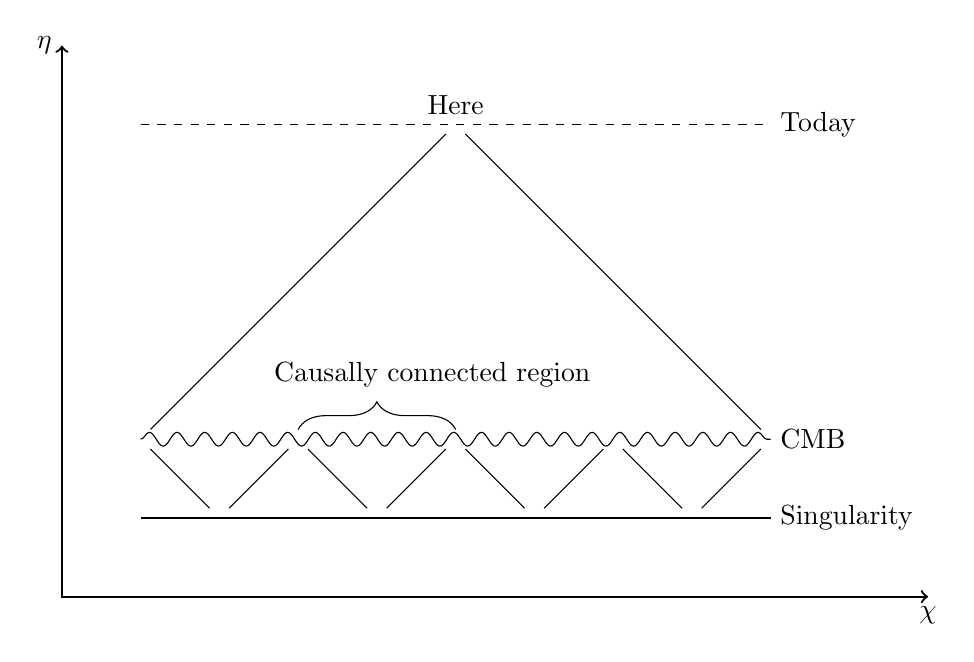
\begin{tikzpicture}
  \draw [<->,thick] (0,7) node (yaxis) [left] {$\eta$}
  |- (11,0) node (xaxis) [below] {$\chi$};

  % CMB

  % singularity
  \draw[] (1,1) -- (9,1) node [right] {Singularity};
  \draw[decorate,decoration=snake] (1,2) node (CMBl) {}  -- (9,2) node (CMBr) [right] {CMB};
  \draw[dashed] (1,6) -- (9,6) node [right] {Today};

  % causal contacts
  \draw (2,1) node (s1) {};
  \draw (4,1) node (s2) {};
  \draw (6,1) node (s3) {};
  \draw (8,1) node (s4) {};

  \draw (1,2) node (c1) {};
  \draw (3,2) node (c2) {};
  \draw (5,2) node (c3) {};
  \draw (7,2) node (c4) {};
  \draw (9,2) node (c5) {};
  \draw (5,6) node (now) {};

  
  \draw (c1) -- (s1) -- (c2);
  \draw (c2) -- (s2) -- (c3);
  \draw (c3) -- (s3) -- (c4);
  \draw (c4) -- (s4) -- (c5);

  \draw (c1) -- (now) -- (c5);
  \draw (now) node [above] {Here};

  \draw [decorate,decoration={brace,amplitude=10pt}]
  (c2.north) -- (c3.north) node [black,midway,yshift=20pt,xshift=20pt] {Causally connected region};

\end{tikzpicture}

  \caption{Horizon problem.\label{fig:cos:horizon_problem}}
\end{figure}

\begin{figure}
  \centering
  \begin{tikzpicture}
  \draw [<->,thick] (0,7) node (yaxis) [left] {$\eta$}
  |- (11,-5) node (xaxis) [below] {$\chi$};

  % CMB

  % singularity
  \draw[] (1,-4) -- (9,-4) node [right] {Singularity};
  \draw[decorate,decoration=snake] (1,2) node (CMBl) {}  -- (9,2) node (CMBr) [right] {CMB};
  \draw[dashed] (1,6) -- (9,6) node [right] {Today};

  % causal contacts
  \draw (2,1) node (s1) {};
  \draw (8,1) node (s4) {};

  \draw (1,2) node (c1) {};
  \draw (9,2) node (c5) {};
  \draw (5,6) node (now) {};
  \draw (5,-2) node (then) {};

  
  \draw (c1) -- (now) -- (c5);
  \draw (c1) -- (then) -- (c5);
  \draw (now) node [above] {Here};
  \draw (now) node [above] {Here};

\end{tikzpicture}

  \caption{Horizon problem resolved.\label{fig:cos:horizon_problem_resolved}}
\end{figure}

\section{An accelerating universe}
\section{Perturbations}
\section{Statistics of the CMB}
We write a general perturbation to the temperature field of the universe as:
\begin{equation}
  T(t,\vx,\vp) = T(t)\left[ 1+\Theta(t,\vx,\vp) \right]
\end{equation}
Note that the temperature field is anisotropic (i.e.\ has a $\vp$ dependency) on account of the relativistic nature of photons. We may separate this angular dependence by expanding $\Theta$ in spherical harmonics:
\begin{align}
  \Theta(t,\vx,\vp) &= \sum_{\ell=1}^{\infty}\sum_{m=-\ell}^{\ell}a_{\ell m}(t,\vx) Y_{\ell m}(\vp)\\
  a_{\ell m}(t,\vx) &= \int d\Omega Y_{\ell m}(\vp) \Theta(t,\vx,\vp)
  \label{eqn:cos:alm_integral}
\end{align}
We only observe the temperature field here (at $\vx_0$) and now (at $t_0$). By taking sufficiently many measurements in different directions of $\vp$ of the temperature field $\Theta$ we can compute the integral~\eqref{eqn:cos:alm_integral}, to obtain $a_{\ell m}(t_0,\vx_0)$ up to some $\ell_{\max{}}$.\footnote{As a rough guide, if one has $N_\mathrm{pix}$ independent pixels, there are ${(\ell_{\max{}}+1)}^2$ different $a_{\ell m}$'s to measure, so $\ell_{\max{}} \sim \sqrt{N_\mathrm{pix}}$.}

In general, theories do no predict specific values of $a_{\ell m}$, but merely tell us about the statistical distribution on which they are drawn. At each value of $\ell$, the $(2\ell + 1)$ observations $\{a_{\ell m}:m=-\ell\cdots\ell\}$ are typically independent realisations of the same random variable. Their mean value is zero, but they will have some non-zero variance:
\begin{equation}
  \left\langle a_{\ell m} \right\rangle = 0, \qquad
  \left\langle a_{\ell m} a_{\ell^\prime m^\prime}\right\rangle = \delta_{\ell \ell^\prime} \delta_{m m^\prime} C_\ell
\end{equation}
Note then that the error therefore in the sample variance obeys:
\begin{equation}
  \left( \frac{\Delta C_\ell}{C_\ell} \right) = \sqrt{\frac{2}{2\ell+1}}.
\end{equation}
This means that on larger angular scales, we have fewer $a_{\ell m}$'s to use to compute the sample variance, and hence have a larger sample error. This is a manifestation of {\em cosmic variance}, resulting from the fact that we only have one universe to observe. 

Computing the theoretical predictions of these $C_\ell$ is complicated, requiring one to evolve the contents of the universe from some initial early time through the hot big bang era, past the surface of last scattering at recombination and all the way to the sky we see today. Treating this stage fully is beyond the scope of this thesis, but it suffices to say that this is extremely well understood physics, and can be computed using codes such as \CAMB{} in a matter of seconds.

\section{Inflation}
The canonical way to explain this early accelerated phase is via the phnomenon of {\em inflation}.

Scalar fields:

\begin{align}
  \rho &= \frac{1}{2}\dot{\phi}^2 + V(\phi) \\
  P &= \frac{1}{2}\dot{\phi}^2 - V(\phi) \\
  0 &= \ddot{\phi} + 3 H \dot{\phi} + \frac{d}{d\phi}V(\phi)
\end{align}



\clearpage{}

